\subsection{XRF Implementation}

\subsubsection{X-ray source}
To incite fluorescence in heavy elements, a high energetic source is needed, as high energy photons is needed to knock their electron out of their orbit. To achieve this a x-ray tube with an Ag anode with an output spectrum as seen in figure \ref{fig:AgSpectra} is recommended. The high energy of the peaks enable the source to achieve fluorescence from elements up to Ag (Z=47), with lesser efficiency up to Sm (Z=62, 40keV).

\begin{figure}[htb]
	\centering
	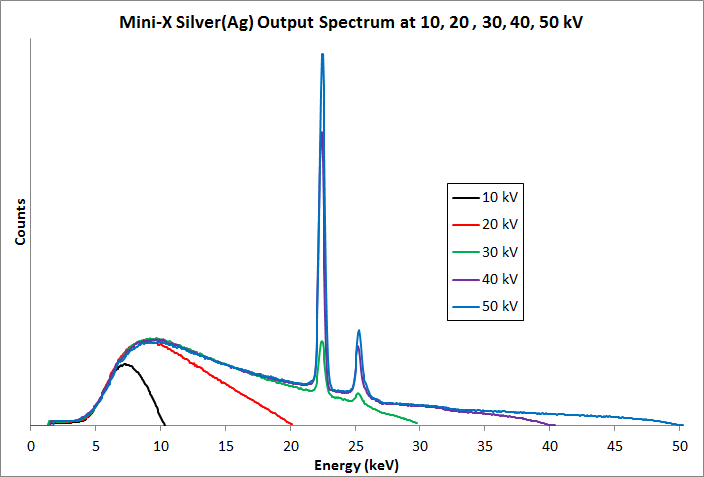
\includegraphics[width=0.75\textwidth]{figures/XRF/minix50_ag6.png}
	\caption{Output spectrum for a x-ray tube using an Ag anode at different voltages.\citep{AmptekSource}}
	\label{fig:AgSpectra}
\end{figure}

The lower end of the energy spectrum is caused by bremsstrahlung in the anode, and is not of much use as it provides little additional resulting fluorescence. The low end is also scattered and will provide a significant noise source for the lower energies. This is particularly undesirable as the lighter elements low energy fluorescence, are also heavily attenuated by the water they are dissolved in. To adjust the spectrum an Al filter can be used to attenuate the lower energies, as seen in figure \ref{fig:AgSpectraFilt}.

\begin{figure}[htb]
	\centering
	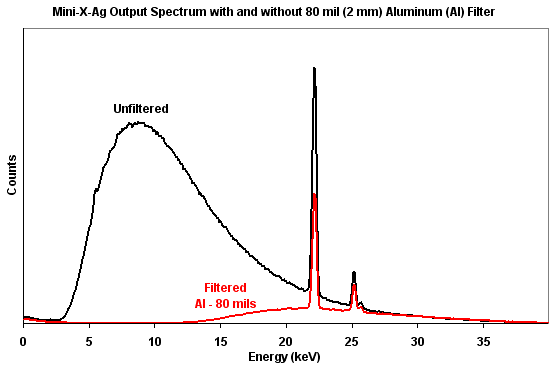
\includegraphics[width=0.6\textwidth]{figures/XRF/minix_Fil.png}
	\caption{Filtered and unfiltered Ag x-ray tube spectrum at 40keV. \citep{AmptekSource}}
	\label{fig:AgSpectraFilt}
\end{figure}


The output spectrum of the x-ray tube have to significant peaks at ~23keV and ~25keV. This is the characteristic lines of Ag when subjected to electron radiation. Knowing these line enables us to take them into account as they will show up as noise in measurements. Focusing on the remaining peaks, and using equation \ref{eq:ComtonEQ}, the Compton scattering resulting from the incident spectrum can be estimated in figure \ref{fig:AgSpectraCompton}.

\begin{figure}[htb]
	\centering
	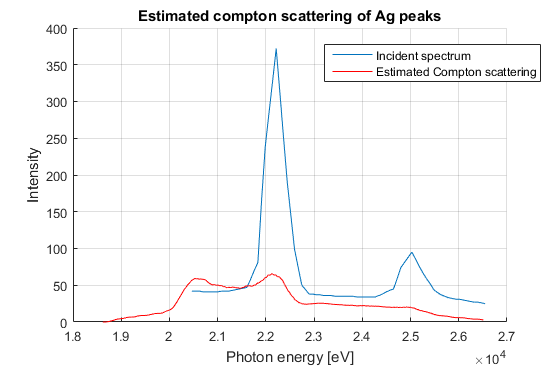
\includegraphics[width=0.6\textwidth]{figures/XRF/estComptonAgPeaks.png}
	\caption{Estimated Compton scattering of the source spectrum.}
	\label{fig:AgSpectraCompton}
\end{figure}

The resulting noise peaks from Compton scattering lies between 20keV and 22.5keV. These will overlap with the $K_\alpha$ of Pd (Z=46, $K_\alpha$ at 21.1keV) and Ag (Z=47, $K_\alpha$ at 22.1keV).
To maximise the amount of x-rays that reach the sample a collimating polycapillary lens should be used between the source and the sample.

\paragraph{Instrument}
Creating the high voltage needed for the instrument a voltage multiplier can be used. The entire instrument can be realized (including high voltage powersupply) with\citep{AmptekSource}:\\
Mass: 360g\\
power: 9W (at max output intensity)\\
Volume: $272.24cm^{3}$\\
The listed weight and volume is without additional protection from the high pressure environment.

\subsubsection{X-ray detector}
When considering the detector the range of encountered photons should be considered. The lighter elements $K_\alpha$ lines are only a few hundred keV apart, to differentiate these a suitable resolution is needed. Detectors also do not perform equally across all energies. The lower limit of the detector is determined by the detector window, as low energy photons are quickly attenuated. The higher limit is determined by the detector material. If we used a polycapillary lens, a window of 25um Be can be used. The detector material can be chosen as Si, as it provides a greater range than what we expect to achieve fluorescence from. In figure \ref{fig:AmptekDetector} a plot of differing detector can be observed. The resolution of the 25um Be SI-PIN detector is sufficient to distinguish elements heavier than Na Z=11.

\begin{figure}[htb]
	\centering
	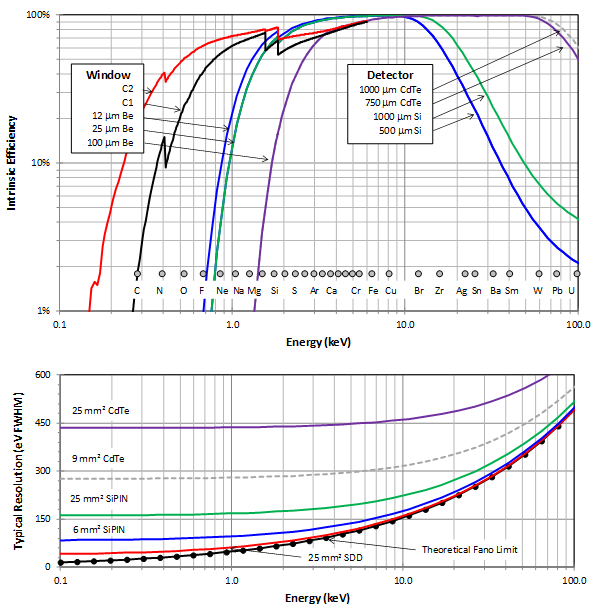
\includegraphics[width=0.8\textwidth]{figures/XRF/EnergyRes.png}
	\caption{Energy resulution and detection ranges of differing detector types.\cite{AmptekDetector}}
	\label{fig:AmptekDetector}
\end{figure}

\paragraph{Instrument}
The instrument, including high voltage power supply and MCA, can be realized with\citep{AmptekDetector}:\\
Mass: 180g\\
power: 4W max, 2.5W typical\\
Volume: $175cm^{3}$\\
The listed weight and volume is without additional protection from the high pressure environment.


\subsubsection{Sample retrieval and configuration}
The sample should be placed as close the polycapillary lens of the detector as possible. As such the sample solution should either be contained in a chamber where one wall is the polycapillary lens of the detector. 
Making another wall, perpendicular to the detector lens, the source lens. The detector is not blinded by the x-ray source, and the source will not lose efficiency by being attenuated by a sample chamber or the surrounding water. Figure \ref{fig:XRFSampleDiagram} show the proposed sample solution. With the sample chamber wall being composed of the source/detector lenses, a sample would have to be pumped into the analyser. And as the lenses can not be changed a certain amount of sample material might be left over after measurement. This can be mitigated through by pumping clean water through the chamber.

\begin{figure}[htb]
	\centering
	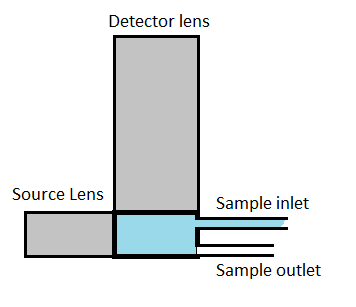
\includegraphics[width=0.5\textwidth]{figures/XRF/SampleDiagram.png}
	\caption{Block diagram showing the position of the sample compared to the source and detector lenses.}
	\label{fig:XRFSampleDiagram}
\end{figure}

If the sample containment chamber is designed to be removable, it should be made of a material with a low x-ray attenuation such as Beryllium. It should also be moved as close to the lenses as possible to reduced loss in the water between sample container and lens.

\subsubsection{XRF analyser Summary}

\paragraph{Detection range} The upper limit of what the XRF analyser can detect is determined by the highest energy photons consistently directed at the sample. This is determined by the source to Ag Z=47.
The lower limit is determined by the detector window to F Z=9. however due to the attenuation of the fluorescent x-rays in the water sample detection of elements lighter than Cobalt seems unlikely, but will have to be determined by empirical test, as it depends on multiple factor such as detector sensitivity and source intensity and spectrum.

\paragraph{Total mass, power and volume} The mass power and volume of the source + detector, without pressure shielding, is as follows:\\ 
Mass: 540g\\
power: 9W max\\
Volume: $447.24cm^{3}$\\

\subsubsection{Additional work}
The polycapillary lenses maximum entrance/exit angles have to be considered for both the source, the detector and the sample. Furthermore empirical testing is needed to determine the exact relationship between source spectrum and detector to determine detection limit in terms of detectable quantity of an element in the sample. The empirical testing would likewise shed light on the piratical upper and lower limits of what elements are detectable with this set-up, when working with an aqueous solution as a sample.
The Source, detector and polycapillary lenses should also be tested to ensure they can withstand the pressure under the ice of Europa.


